

\typeout{Towards Artificial Intelligence for Metaphysics: \\ the Case of the Inconsistency in G\"odel's Ontological Argument}


\documentclass{article}
\usepackage{ijcai15}

% Use the postscript times font!
\usepackage{times}


% the following package is optional:
\usepackage{latexsym} 

\usepackage{amsmath}
\usepackage{xspace}
\usepackage{modallogics}
\usepackage{graphicx,url}
\usepackage{txfonts} % needed for \Diamondblack
\usepackage{float}

\newcommand{\imp}{\rightarrow}
\newcommand{\biimp}{\leftrightarrow}
\newcommand{\allq}{\forall}
\newcommand{\exq}{\exists}
\newcommand{\seq}{\vdash}

\newcommand{\Dia}{\Diamond} % possibly
\newcommand{\BlackBox}{\blacksquare}
\newcommand{\BlackDia}{\Diamondblack}



\title{Towards Artificial Intelligence for Metaphysics: \\ the Case of the Inconsistency in G\"odel's Ontological Argument}
\author{Christoph Benzm\"uller\thanks{German Research Foundation DFG \ldots} and Bruno Woltzenlogel Paleo}
\author{}

\begin{document}

\maketitle

\begin{abstract}
  This paper discusses the discovery of the inconsistency in G\"odel's ontological argument as a success story for artificial intelligence. Despite the popularity of the argument since the appearance of G\"odel's manuscript in 1970, the inconsistency of the axioms used in the argument remained unnoticed until 2013, when it was detected automatically by the higher-order theorem prover LEO-II. Understanding and verifying the refutation generated by the prover turned out to be a time-consuming task, and its completion, as reported here, required the reconstruction of the refutation in the Isabelle proof assistant. The development of an improved syntactical hiding for the embedding technique, utilizing Isabelle's binding notation mechanism, allows the refutation to be presented in a human-friendly way, suitable for non-experts in the technicalities of the higher-order theorem proving. This brings us a step closer to wider adoption of logic-based artificial intelligence tools by philosophers.
\end{abstract}


\section{Introduction}
Without exaggeration Kurt G\"{o}del's ontological
argument for the existence of God \cite{GoedelNotes,ScottNotes} is
amongst the most discussed formal proofs in modern literature. A rich
body of publications -- including very recent ones -- present,
discuss, assess, criticise, modify and improve G\"{o}del's original
work (see e.g.~Sobel~\shortcite{Sobel} and Oppy~\shortcite{sep-ontological-arguments} and the
references therein).  In philosophy lectures at universities the
argument is regularly presented as a masterpiece argument in
metaphysics. Since 2013, when Benzm\"uller and Woltzenlogel-Paleo~\shortcite{J30,C40} first
reported their successful initial computer-assisted
analysis of G\"odel's proof and Scott's variant,
their work has received a media repercussion on a global scale\footnote{A
  small collection of news articles is available at {\scriptsize
    \url{https://github.com/FormalTheology/GoedelGod/blob/master/Press/LinksToNews.md}}},
and numerous bloggers commented on the proof
\cite{fuhrmann15:_blogg_goedel}.

The in-depth computational analysis presented here substantially
extends previous computer-assisted studies of G\"odel's ontological
argument. Similar to the related work \cite{J30,C40} the analysis has
been conducted with automated theorem provers for classical
higher-order logic (HOL) even though G\"odel's proof is actually
formulated in \emph{modal} higher-order logic. To bridge between the two
logics we utilise and further improve the logic embedding
approach \cite{J23,C40}, which has already been employed succesfully in preceding related work.


The novel contributions reported in this paper include the following:

\begin{itemize}
\item A detailed analysis of the inconsistency of G\"{o}del's
  \shortcite{GoedelNotes} original version of the proof is presented
  for higher-order modal logics KB and K (with possibilist and
  actualist first-order quantifiers). The extraction, reconstruction
  and verification of an informal, human intuitive argument has been
  an open problem since the first detection of this inconsistency by
  Benzm\"uller and Woltzenlogel-Paleo \shortcite{C40} with the LEO-II prover. 
  The experiments reported here led to the discovery of a surprisingly accessible
  understanding of this inconsistency which is philosophically
  profound and which has not been presented yet in the
  literature. The detection of this inconsistency in combination with
  the work reported here thus demonstrates that artificial intelligence systems -- 
  particularly higher-order automated
  theorem provers -- are capable of assisting in the discovery and ellucidation of
  \emph{new} and philosophically relevant knowledge. 
\item Another open question has been whether the final theorem T3 \textit{``Necessarily, there
    exists God''} could eventually be proved fully automatically
  directly from the axioms alone. In \shortcite{C40}, the provers had only succeeded in proving 
  T3 from intermediate argumentation steps (lemmata). Here we report that, by using a more efficient new
  embedding for the higher-order modal logic S5, T3 can be directly proven from Scott's version of the axioms, which are consistent. The fully automatic proof has been
  generated by the theorem prover \textsc{Leo-II}~\cite{C26} and
  subsequently verified in the proof assistant
  Isabelle/HOL~\cite{NPW02}.
\item A third open challenge the verification in Isabelle/HOL of the modal
  collapse \cite{Sobel}, which is one of the most strongly criticised
  `side-effects' of G\"odel's and Scott's variants of the proof. In previous work
  the modal collapse has been derived by the provers
  \textsc{Satallax} \cite{Satallax} and \textsc{Leo-II}, but a fully automatic
  verification in the highly trusted Isabelle/HOL still failed. 
  Now, with the more efficient embedding for S5, this verification has been done. 
\item On the technical side, we present a significantly improved
  syntax representation of G\"odel's resp.~Scott's proof in
  Isabelle/HOL. In fact, we demonstrate that a nearly perfect match
  between the original pen and paper presentations and our encoding in
  Isabelle/HOl is feasible. This is clearly an important prerequisite
  for promoting the theorem proving technology employed here to a wide community of
  philosophers, who are not necessarily experts in automated reasoning or higher-order logic.
\item On the other hand, we
  also point to several technical challenges which, at least for the
  moment, still restrain non-expert users of these systems from
  independently conducting similar experiments in computational
  metaphysics as reported here and in previous work. 
% Technical issues detected within Isabelle-Sledgehammer; room for improvements
\end{itemize}


First successful applications of theorem proving technology in
metaphysics were reported by Oppenheimer and
Zalta~\shortcite{oppenheimera11}, who coined the term \textit{Computational Metaphysics} for this new research area and employed the first-order
\textsc{Prover9} \cite{Prover9} in their experiments. Later on, Rushby~\shortcite{rushby13} used the proof assistant \textsc{PVS} \cite{PVS}. Common to both
works is a significant amount of proof-hand-coding work as well as their
focus on a non-modal formalization of St. Anselm's~\shortcite{Anselm} simpler 
and older ontological argument. 
None of these previous works formalises and automates variants of \emph{higher-order} and \emph{modal} logics, which are, however, crucial
for G\"{o}del's more complex ontological argument.


\section{A Brief History of the Argument}

St. Anselm's ontological argument \cite{Proslogion} can be regarded as the ancestor of modern ontological arguments such as G\"odel's. In the millenium between Anselm and G\"odel, many philosophers modified and arguably improved Anselm's argument. Of particular importance to G\"odel was the work of Leibniz \cite{ToDo}. 
G\"odel's manuscript (Figure \ref{GoedelScript}) can be considered a translation of Leibniz's presentation of the argument into modern modal logic. G\"odel shared his manuscript with Scott, who shared a slightly different version with a larger public. Scott's version of the axioms and definitions, formalized in Isabelle, is shown in Figure \ref{ScottS5}. The main difference to G\"odel's version is the addition of a conjunct in the definition of \emph{essence}. G\"odel's different definition of essence can be seen either in his manuscript (Figure \ref{GoedelScript}) or, in more modern notation, in the Isabelle formalization shown in Figure \ref{nconsistencyIsabelleK}. For Scott, an essential property of an individual must be possessed by him/her. For G\"odel, this is not required. This difference has been considered inessential and merely an oversight by many. For instance, Hazen 1998, p.365 \cite[p.365]{Hazen1998} states that ``G\"odel left this clause out in [11], but this appears to have been an oversight--it is included in related manuscripts''. However, the omitted conjunct is in fact crucial. Without it, G\"odel's original axioms are inconsistent. With it, Scott's axioms are consistent.


% There is reason to believe that the omission was more than just an oversight. As pointed out by Fuhrmann \cite{Fuhrmann2005}, ``G\"odel vermerkt diese Konsequenz [dass aus der Definition unmittelbar folgt, da\ss alle wesentlichen Eigenschaften notwendig äquivalent sind] in einer Fußnote zur Definition. Die Definition selbst aber l\"a{\ss}t im Definiens das Konjunkt $Xx$ aus. Ohne das Konjunkt folgt jedoch die Konsequenz nicht. Es ist deshalb naheliegend anzunehmen, da\ss G\"odel die Definition so beabsichtigte, wie sie hier notiert ist und wie G\"odel sie selbst in fr\"uheren Notizbucheintragungen formuliert hat.''\footnote{Our translation: ``G\"odel remarks this consequence [that the definition of essence entails that all essences are necessarily equivalent] in a footnote to the definition. The definition, however, omits the conjunct. ... ToDo''} 
% \marginpar{ToDo: check Fuhrmann's claim. He may be pointing out a second mistake by Gödel.}

For more than four decades, the serious consequences of G\"odel's mistake remained unnoticed, despite intense activity focused on criticizing his argument. Especially since the discovery by Sobel \cite{Sobel} that a modal collapse is entailed by G\"odel's (or also Scott's) axioms, several variants have been proposed \cite{Anderson,AndersonGettings1968,Hajek,Hajek2,Hajek3,Bjordal} attempting to avoid the modal collapse. Many of these variants omit the crucial conjunct in the definition of essence as well\footnote{As these variants also change other axioms, on which the inconsistency of G\"odel's axioms depends, it is not necessarily the case that these variants are also inconsistent.}. Opponents of the argument (e.g. Oppy \cite[p.226/227]{Oppy1996} \cite[p.364]{Oppy2000} \cite[p.1068]{Oppy2008}) have also proposed parodies and other criticisms, referring to variants where the conjunct is omitted.





%  Particularly interesting
% from the perspective of this paper is that many literature
% contributions unfortunately work with or refer to G\"odel's original
% definition of essence
% $$ todo $$
% This original version avoids the conjunct added by Scott expressing
% that essential properties of an individual should be possessed by the
% individual. 

% We give here a list of examples:
% \begin{itemize}
% \item Anderson and Getting's 1996, p. 168 \cite[p.168]{AndersonGettings1968}
%   use essence without conjunct.
% \item  
% \item Look???, p. 514
% % \item Oppy 1996, p.226-227 \cite[p.226/227]{Oppy1996}, Oppy 2000, p. 364
% %   \cite[p.364]{Oppy200}, Oppy 2008, p. 1068 \cite[p.1068]{Oppy2008}:
% %   Oppy uses: ``A is an essence of x iff for every property B, x has B
% %   neces- sarily iff A entails B'' (this is from Anderson's
% %   emendation). Check is this leads to inconsistency as well. In this
% %   case we may write something like: 

% %  Oppy presents an critical
% %   assessment in order to conclude that G\"odel's argument fails to
% %   convince. Oppy apparently does not see that he is assessing an
% %   inconsistent axiom system (and he in fact creates adaptations that
% %   suffer the same problems).
% % \item 
% \end{itemize}








\section{Automating HOML in HOL}

Logic textbooks \cite{ToDo: which} commonly utilize classical higher-order logic (HOL)
\cite{Church} as a meta-language to introduce the syntax and the
semantics of object logics of interest, in which reasoning
problems in concrete application domains can be modeled and solved
with pen and paper. In fact, this approach can also be followed for even very challenging
object logics to
enable interactive and automated theorem proving with existing theorem provers for classical
higher-order logic.

% Just as commonly the case in logic textbooks, in the embeddings
% approach classical higher-order logic is utilised as a meta-language
% to encode the syntax and the semantics of object logics in which the
% proof problems of interest are then modeled in. Modulo the embedding
% state of the art automated theorem provers for classical higher-order
% logic can then be utilised as object logic reasoning tools.

For a computational analysis of G\"odel's ontological argument in this
approach the embedding of higher-order modal logics (HOML) such as K,
KB and S5 with various domain conditions (possibilist and actualist)
is required. This idea has been successfully followed in related work
\cite{C40}. The embedding of higher-order modal logic is in fact
straightforward. Formulas in HMOL are \emph{lifted}, translated to predicates
over worlds, which are themselves explicitly represented as
terms. The logical constants of HMOL are translated to HOL terms in such a way that, for instance, 
%$\neg \varphi$, $\varphi\vee\psi$
$\Box \varphi$ and $\Diamond \varphi$ are mapped, respectively, to the HOL formulas $\forall w. (r w_0 w) \imp (\varphi w)$ and $\exists w. (r w_0 w) \wedge (\varphi w)$. This form of embedding is precisely the well-known standard translation \cite{Ohlbach,ModalLogicPatrickBlackburn},
which is here (intra-logically) realized in HOL by stating a set of
equations defining the logical constants (Fig. ~\ref{QMLS5}). The resulting object logic is the HOML K with rigid terms and constant domains (possibilist quantifiers). Other logics (e.g. KB, S5) can be embedded by adding axioms that restrict the accessibility relation $r$. Varying domains and actualist quantifiers can be simulated by means of an existence predicate, which can be used to guard the quantifiers. Therefore, the embedding approach is very flexible.


\subsection{Improved Embedding for \SFiveU}

The modal logic \SFive requires that the accessibility relation be reflexive, symmetric and transitive. The usual approach to embed \SFive would be to use the standard translation for K described above and state these additional conditions as three HOL axioms: 
\begin{itemize}
\item Reflexivity: $\forall x. (r~x~x)$
\item Symmetry: $\forall x. \forall y. (r~x~y) \rightarrow (r~y~x)$ 
\item Transitivity: $\forall x. \forall y, \forall z. (r~x~y) \wedge (r~y~z) \rightarrow (r~x~z)$
\end{itemize}

We consider here a modal logic that we call \SFiveU, which is characterized by the following condition on the accessibility relation:
\begin{itemize}
\item Universality: $\forall x. \forall y. (r~x~y)$
\end{itemize}

It is easy to see that \SFiveU is at least as strong as \SFive: universality entails reflexivity, symmetry and transitivity. \SFiveU is, in fact, \emph{strictly stronger} than \SFive. \SFiveU only admits complete\footnote{A graph is \emph{complete} iff there is a directed edge connecting every ordered pair of vertices.} frames, whereas \SFive admits non-complete frames as long as all their components are complete.

For \SFiveU, an improved embedding is possible. Universality implies that the guarding predicates in the definitions of $\Box$ and $\Diamond$ always hold. Therefore, they can be omitted and the accessibility relation can be dispensed altogether. The modal operators can then be defined merely as:
\begin{itemize}
\item $\BlackBox \varphi \equiv \forall w. (\varphi w)$ 
\item $\BlackDia \varphi \equiv \exists w. (\varphi w)$
\end{itemize}

The improved embedding of \SFiveU in Isabelle is shown in Fig.~\ref{QMLS5}.
\begin{figure}
\centerline{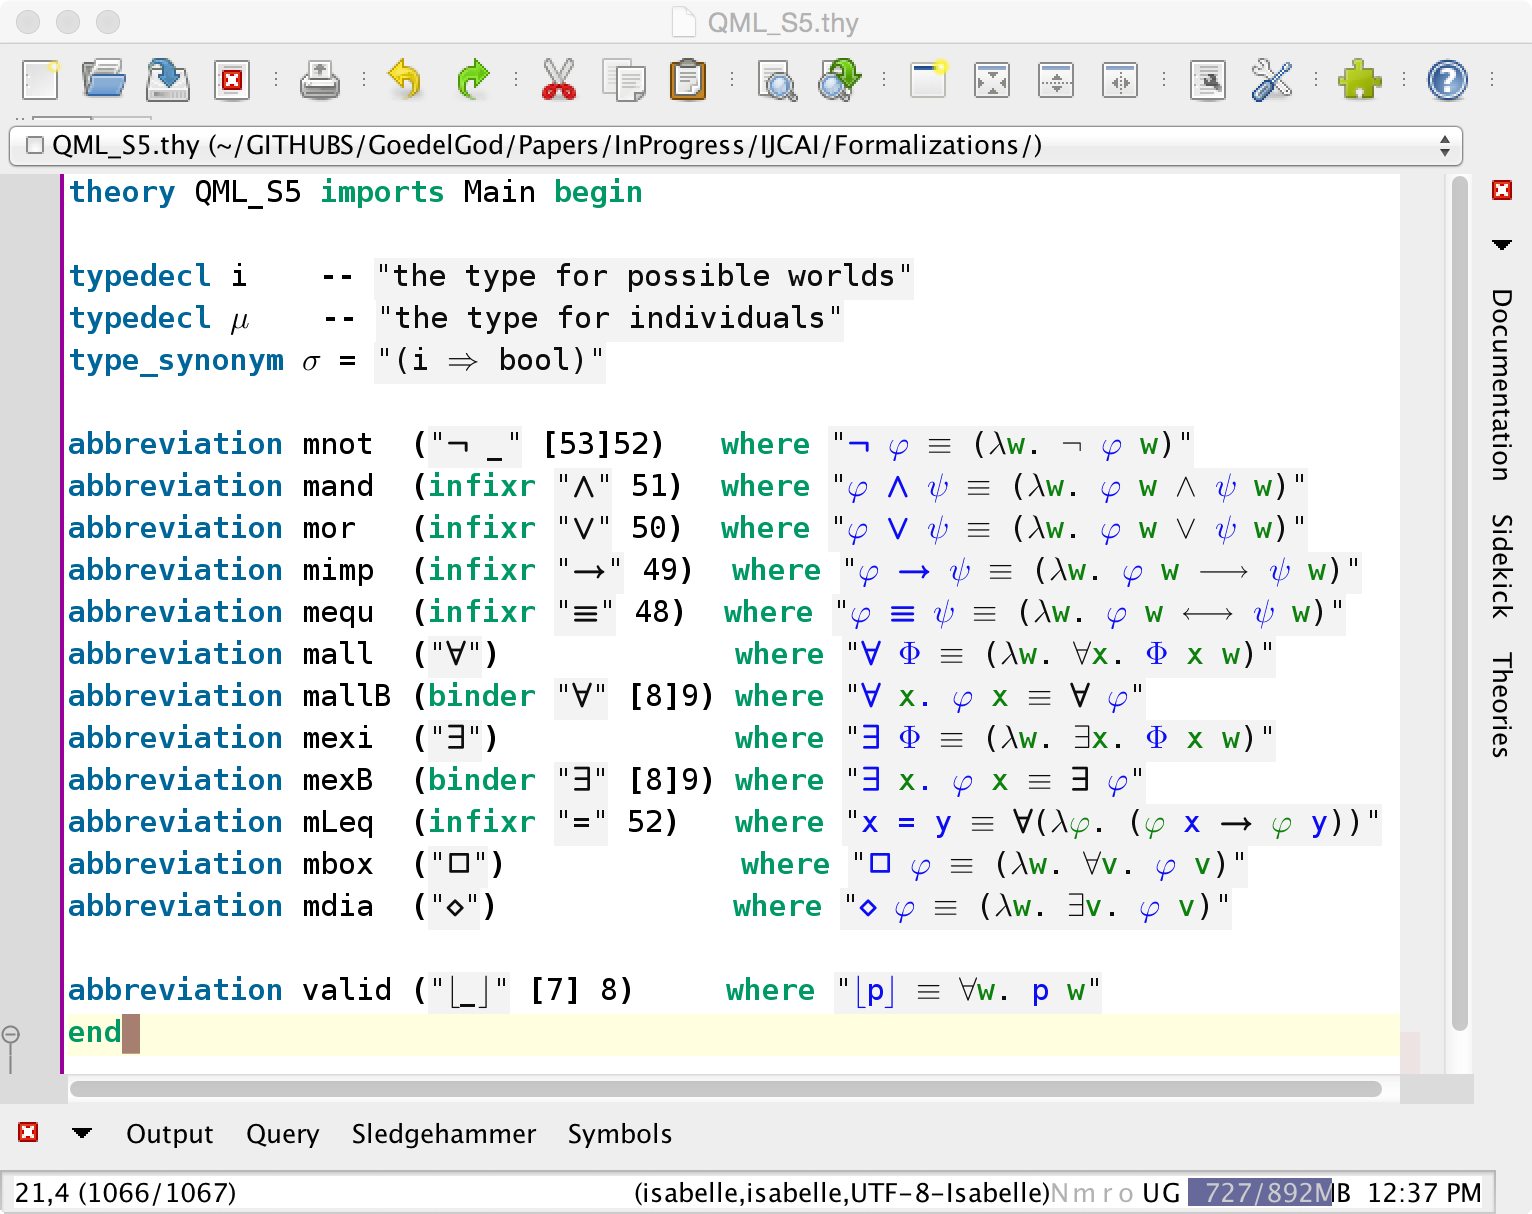
\includegraphics[width=\columnwidth]{./Images/QMLS5.png}}
\caption{Improved Embedding of \SFiveU} \label{QMLS5}
\end{figure}

\SFiveU is only slightly stronger than \SFive. Most importantly, $\vDash_{\SFive} \varphi$ iff $\vDash_{\SFiveU} \varphi^{U}$, where $\varphi^U$ is obtained from $\varphi$ by replacing all $\Box$ and $\Dia$ by, respectively, $\BlackBox$ and $\BlackDia$. Therefore, \SFiveU can be considered as adequate for metaphysics as \SFive (cf. \cite{Mattey}, \cite[p. 127]{WilliamsonModalLogicAsMetaphysics}, \cite[ToDo]{DunnHardegree}). 


With the improved embedding for \SFiveU, the main theorem T3 can be derived from Scott's version of the axioms fully automatically. The
intermediate argumentation steps as not needed anymore to support the
prover.  This is shown in Fig.~\ref{ScottS5}. There it is also shown that the modal collapse can now be verified in
Isabelle/HOL with Meson. In previous work, with a less efficient embedding for \SFive, this failed.
\begin{figure}
\centerline{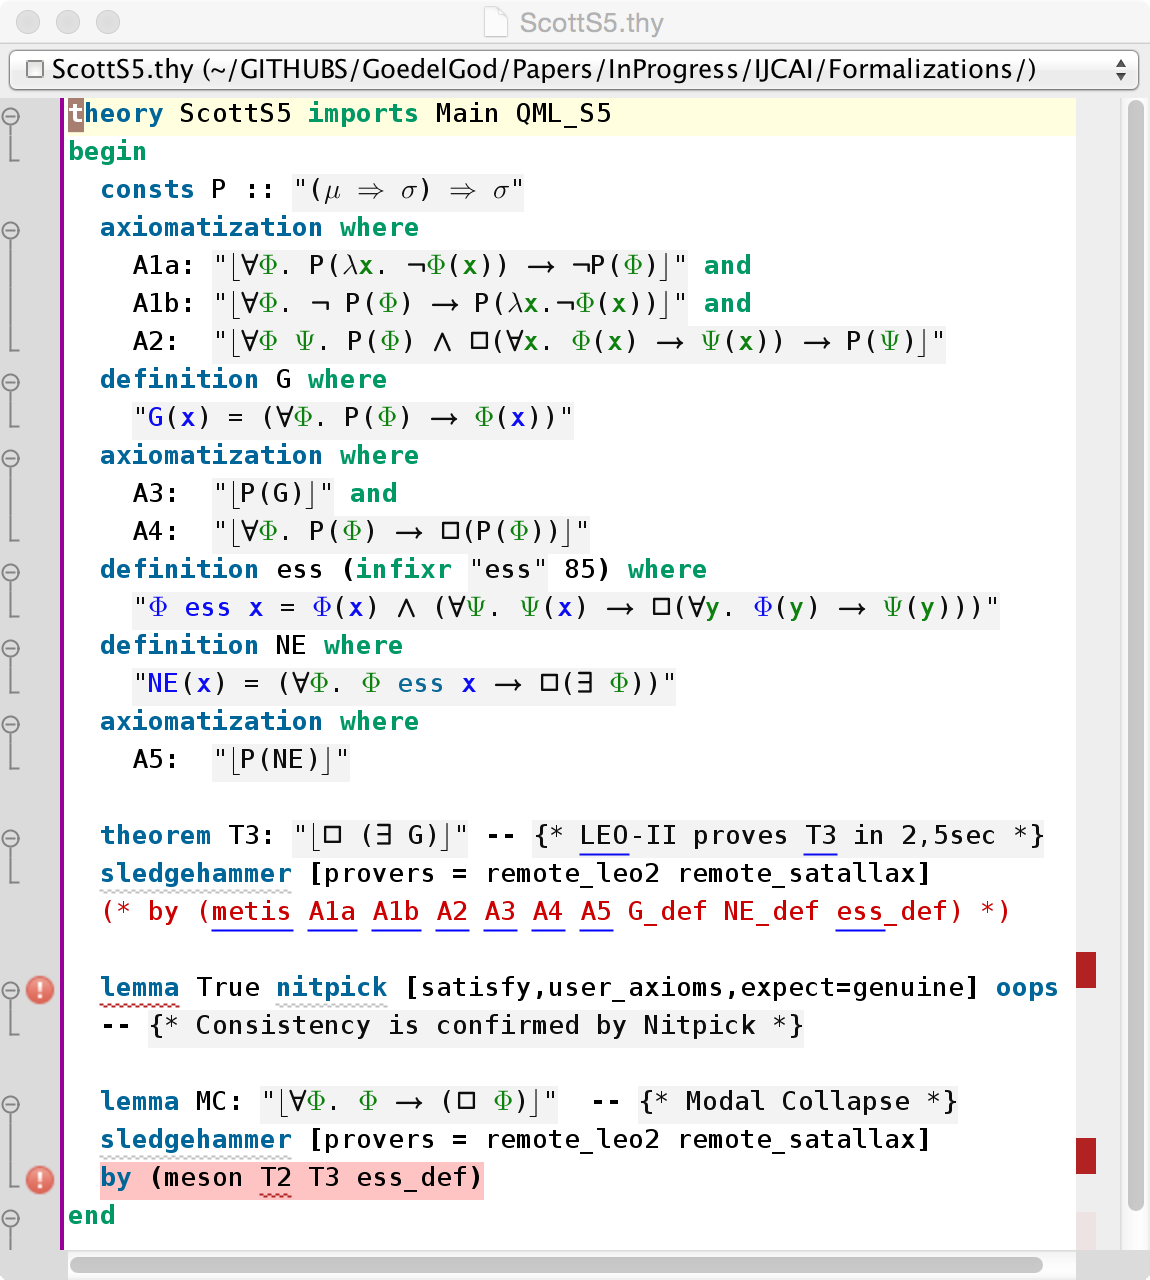
\includegraphics[width=\columnwidth]{./Images/ScottS5.png}}
\caption{Full Automation of T3 and MC in \SFiveU } \label{ScottS5}
\end{figure}
\marginpar{ToDo: this picture has to be replaced by one without Isabelle errors}




\section{Intuitive Inconsistency Argument}
\subsection{LEO-II's Inaccessible Inconsistency Proof}
Tell the story (here or earlier). Show parts of LEO proof.  Inaccessible, but relevant knowledge
is contained.
\begin{figure*}
\centerline{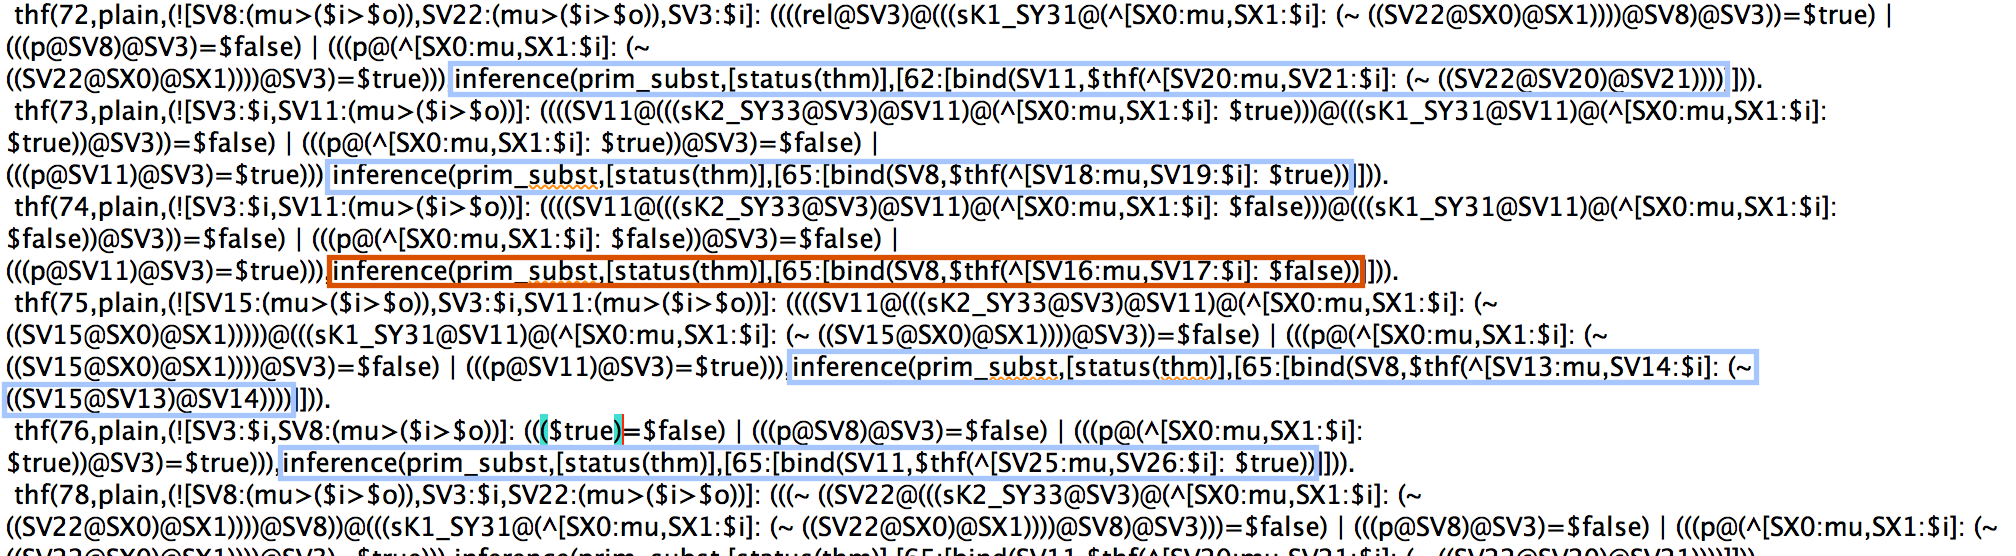
\includegraphics[width=\textwidth]{./Images/LEO-Proof.png}}
\caption{Primitive substitution in LEO-II generates candidates for the
empty property.} \label{LEO-Proof}
\end{figure*}
LEO-II's resolution proof is human unintuitive. However, it contained
relevant hints to the empty property (cf. Fig.~\ref{LEO-Proof}).

\subsection{Argument Reconstruction in Isabelle}
Present the argument informal and in Isabelle (see
Fig.~\ref{InconsistencyIsabelleK}). Easy to understand in 
in KB and KT, slightly harder in K.
\begin{figure}
\centerline{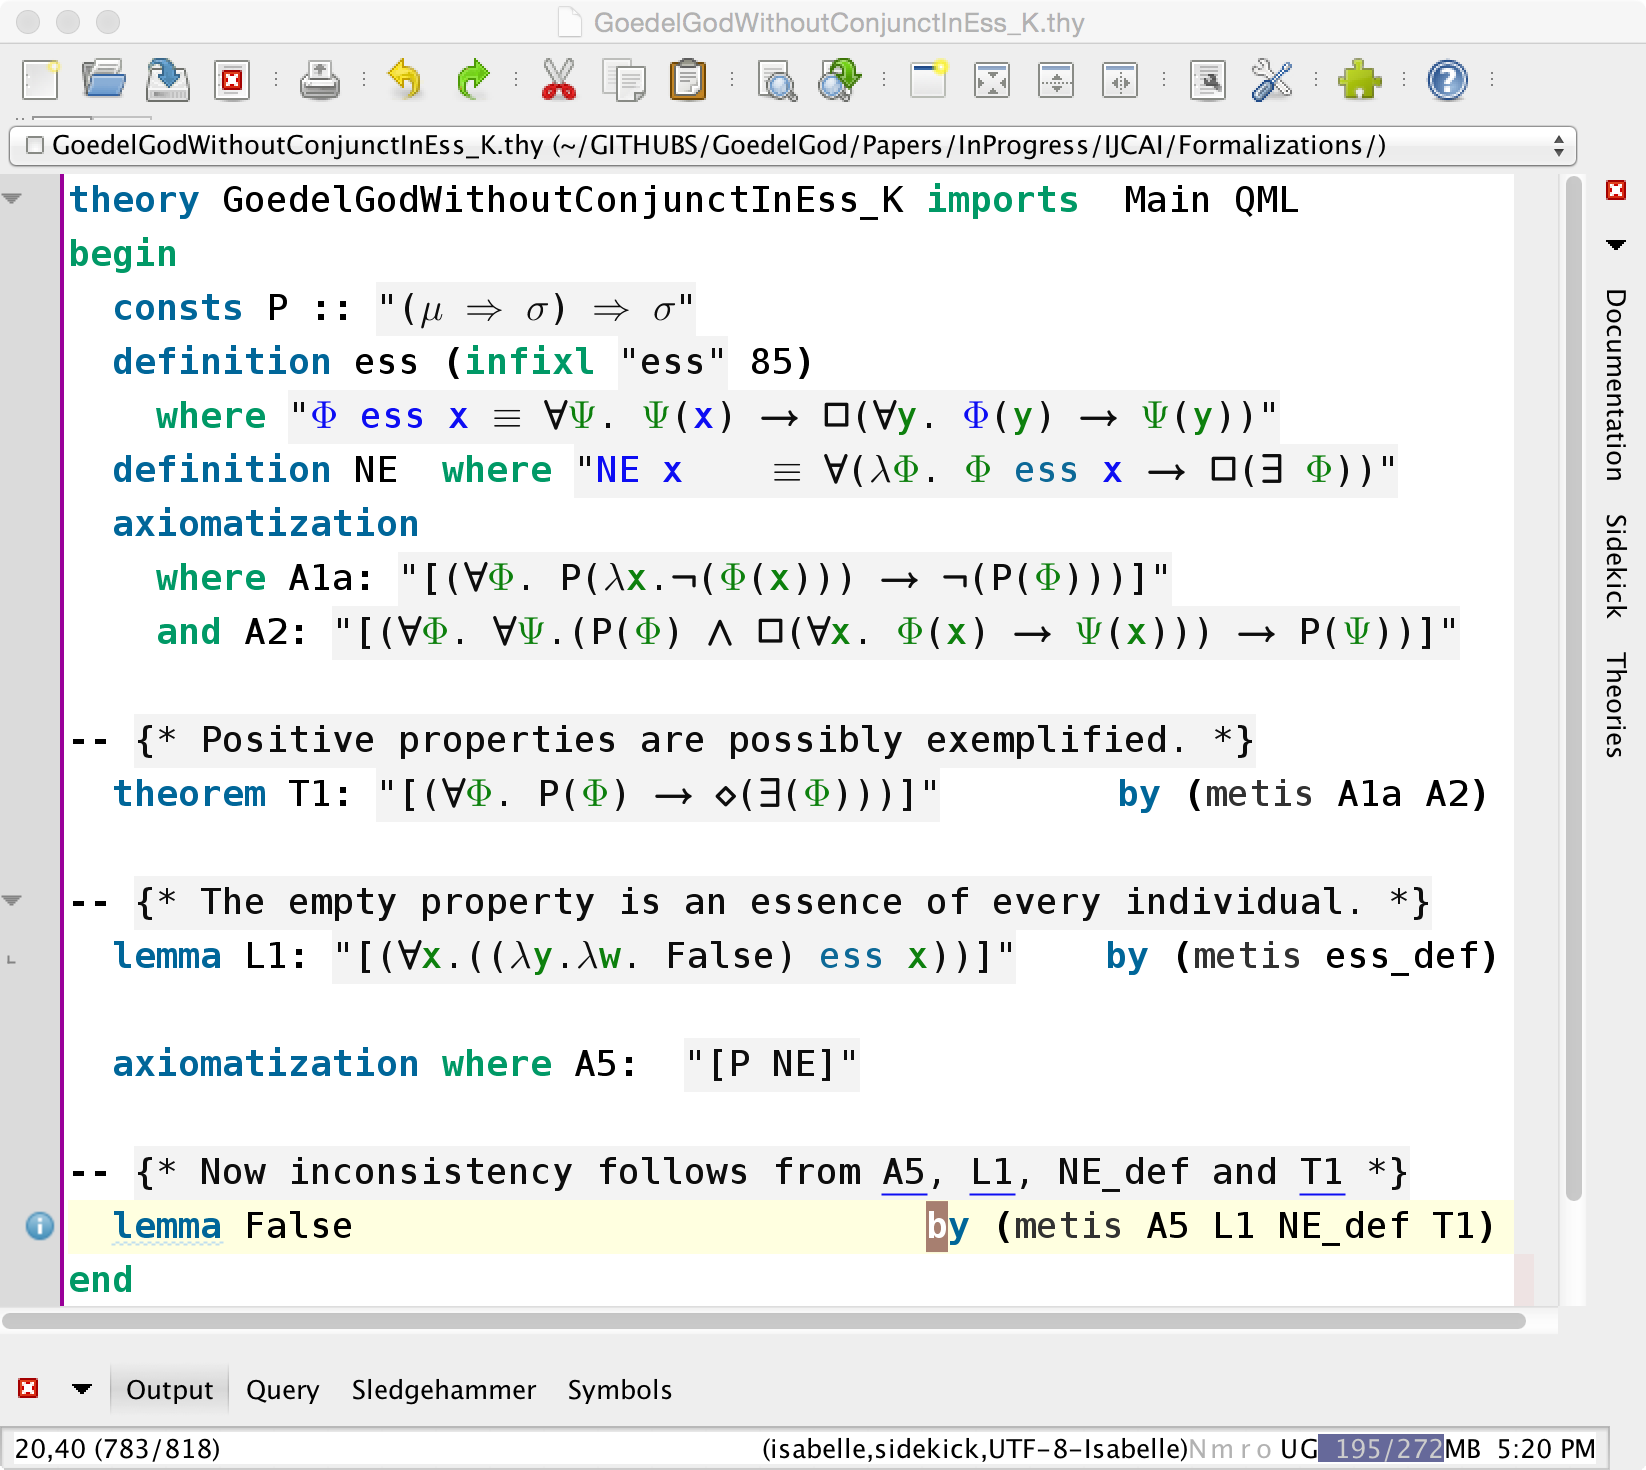
\includegraphics[width=\columnwidth]{./Images/InconsistencyIsabelleK.png}}
\caption{Reconstruction of inconsistency in Isabelle/HOl..} \label{InconsistencyIsabelleK}
\end{figure}





\section{Conclusion}


Good improvement (technical sense), Sledgehammer can still be improved
(LEO-II finds inconsistency when call directly in THF Syntax, but not
from within Isabelle). Without independent experiments directly in THF 
the inconsistency would thus not have been detected.


As we show in this paper using this notion of essence
leads to an inconsistent axiom system, which in a classical setting of
course deserves no further attention, since from an inconsistent
system everything can be concluded, including God's existence and
non-existence simultaneously. In other words, these literature
contributions discuss variants of the argument which from a classical
logical perspective do not deserve any further attention.


\section*{Acknowledgments}

Will be added at a later point.

%German Research Foundation DFG, Chad Brown


\begin{figure*}
\centerline{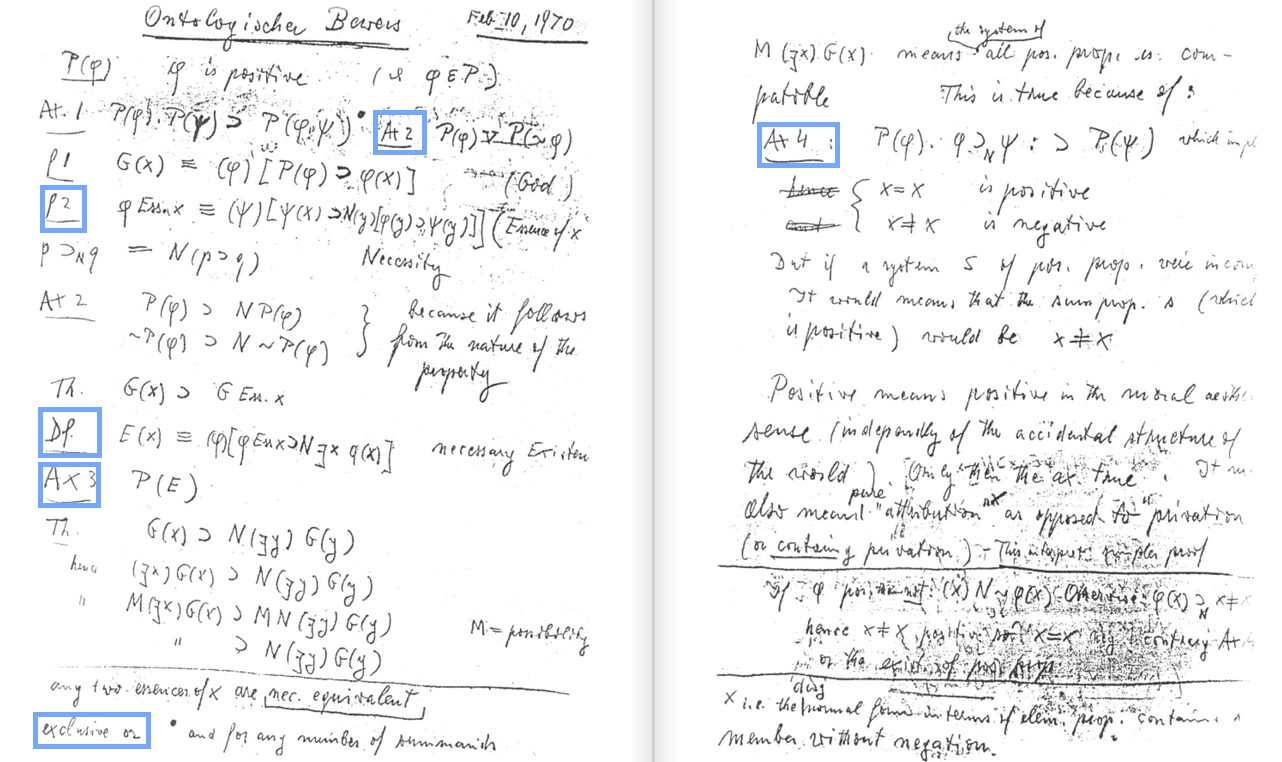
\includegraphics[width=\textwidth]{./Images/Manuscript2.png}}
\caption{G\"{o}del's manuscript, with mutually inconsistent axioms and definitions highlighted.} \label{GoedelScript}
\end{figure*}


\appendix


%% The file named.bst is a bibliography style file for BibTeX 0.99c
\bibliographystyle{named}
\bibliography{Bibliography}

\end{document}

